\chapter{التغير العالمي والمحيط الحيوي}\label{ch:b2:global-change}

بين سنتي 1851 و1858 جال هنري ثورو غابات ومروج
كونكورد في ماساتشوستس، ودوّن اليوم الذي أزهر فيه أول مرة كل
من نحو خمسمئة نبات. وبعد قرن ونصف،
عاد نباتيون إلى الأماكن نفسها بدفاتره. فالتوت الأزرق
الشجيري الذي رآه ثورو ينفتح في 11 أيار صار ينفتح في
12 نيسان؛ والفلورا كلها تزهر، وسطيًا، قبل عشرة أيام
مما كانت في زمنه، على وتيرة ربيع صار أدفأ بمقدار \qty{2.4}{\celsius}؛
وربع أنواعه زال من كونكورد --- لا
عشوائيًا، بل تلك التي لم يستطع إزهارها تتبع
الحرارة. وقد أعطت الفصول السابقة الآلة: دورات
\cref{ch:b2:biogeochemical-cycles}، وانتقاء وانجراف
\cref{ch:b2:population-genetics}، ومنافسة وانتواع
\cref{ch:b2:speciation}، وترب \cref{ch:b2:living-soil}.
وهذا الفصل يضع رقمًا على ما يحدث للأحياء
إذ يغير نوع واحد كيمياء الهواء والبحر: كم
احترارًا لكل طن كربون، وكم يومًا من الربيع لكل
درجة، وكم مترًا صعودًا، وكم حمضًا في البحر، وكم
نوعًا في الهكتار يضيع --- وماذا تقول الأعداد عن
القرن القادم.

\section{التغير الفيزيائي}

\begin{proposition}[الاحترار يتناسب مع الانطلاقات المتراكمة]\label{prop:b2:global-change:tcre}
\index{احترار عالمي}\index{انطلاقات متراكمة}\index{ميزانية الكربون}\index{أثر الدفيئة}
ثاني أكسيد الكربون يمتص الأشعة تحت الحمراء التي تصدرها الأرض ويعيد
جزءًا منها؛ فمزيد من \ensuremath{\mathrm{CO_2}} يعني سطحًا أدفأ، بنحو
\qty{3}{\celsius} لكل مضاعفة متى لحقت المحيطات
(وهي \emph{الحساسية المناخية}). ولمّا كانت استجابة الحرارة
للمقدار \ensuremath{\mathrm{CO_2}} لوغاريتمية في التركيز في حين يهبط \omterm{prop:b2:biogeochemical-cycles:carbon}{الكسر المحمول
جوًا} من الانطلاقات كلما ارتفع التركيز، تلاشى
الانحناءان تقريبًا، فصار الاحترار المتوسط العالمي، بتقريب
جيد، \emph{خطيًا في كمية الكربون المنطلقة
المتراكمة}، مهما كان التوقيت:
\[
\Delta T \approx \lambda\,C_{\text{المتراكم}}, \qquad \lambda \approx
\qty{1.65}{\celsius} \text{ لكل } \qty{1000}{GtC}
\]
(أي \qty{0.45}{\celsius} لكل \qty{1000}{Gt} من \ensuremath{\mathrm{CO_2}}). ونحو
\qty{700}{GtC} انطلقت منذ 1850 قد أدفأت الكوكب
\qty{1.2}{\celsius} --- والعلاقة تعطي كل هدف
ميزانيته: فالهدف \qty{1.5}{\celsius} يتيح نحو \qty{900}{GtC} إجمالًا،
أي \qty{200}{GtC} فوق ما انطلق، وهي عشرون سنة بالمعدل
الحالي. والاحترار غير متساوٍ: فهو ضعف المتوسط على اليابسة
وثلاثة أضعافه في القطب الشمالي؛ والليالي أكثر من الأيام؛ ويأتي
مع الباقي --- مطر أشد وجفاف أطول، ومستوى بحر
يرتفع \qty{4}{mm} في السنة، وجليد أصغر بالخُمس في
الصيف، ومحيط امتص \qty{90}{\%} من الحرارة و
ربع الكربون.
\end{proposition}
\begin{proof}[شواهد]
وُجد التناسب في نماذج مناخية بكل درجات
التعقيد وأكده السجل الملحوظ: فرسم
الاحترار منذ 1850 في مقابل \omterm{prop:b2:global-change:tcre}{الانطلاقات المتراكمة} يعطي خطًا مستقيمًا
عبر العقود. \omterm{prop:b2:global-change:tcre}{وأثر الدفيئة} نفسه يُقاس
من المدار: إذ ترى السواتل الأشعة تحت الحمراء التي تصدرها الأرض وقد قُصّت منها
حزم امتصاص \ensuremath{\mathrm{CO_2}} والميثان وبخار الماء،
وقد تعمّق القص بين 1970 و2020 بالضبط
بالمقدار الذي يتنبأ به ارتفاع هذه الغازات. والنظائر
والأكسجين الهابط في \cref{ch:b2:biogeochemical-cycles} تربط
\ensuremath{\mathrm{CO_2}} الزائد بالوقود الأحفوري.
\end{proof}

\begin{omfigure}
\begin{tikzpicture}
\begin{axis}[
  width=0.88\linewidth, height=5.6cm,
  axis x line=bottom, axis y line=left,
  xmin=1845, xmax=2030, ymin=-0.3, ymax=1.5,
  xlabel={العقد}, ylabel={الاحترار (\unit{\celsius}) منذ 1850--1900},
  xlabel style={font=\small, at={(axis description cs:0.5,-0.13)}, anchor=north},
  ylabel style={font=\small},
  tick label style={font=\small}, xtick={1850,1900,1950,2000}, ytick={0,0.5,1,1.5},
  scaled x ticks=false, x tick label style={/pgf/number format/1000 sep=},
  clip=false,
]
\addplot[ybar, bar width=7pt, fill=omThm!50, draw=omThm] coordinates {
(1855,0.00) (1865,-0.04) (1875,0.02) (1885,-0.06) (1895,-0.02) (1905,-0.10) (1915,-0.06) (1925,0.05) (1935,0.15) (1945,0.25) (1955,0.15) (1965,0.15) (1975,0.18) (1985,0.40) (1995,0.55) (2005,0.78) (2015,1.02) (2023,1.28)};
\node[font=\scriptsize, anchor=west, align=left] at (axis cs:1850,1.2) {كل عمود: متوسط عقد؛ والأخير 2020--2024\\ \qty{700}{GtC} منطلقة، و$\qty{1.65}{\celsius}/\qty{1000}{GtC}$: أي \qty{1.2}{\celsius}};
\end{axis}
\end{tikzpicture}

{\small الحرارة السطحية المتوسطة العالمية بالعقد، نسبةً إلى
النصف الثاني من القرن التاسع عشر. والعقود الأربعة الأخيرة
سجّل كل منها رقمًا قياسيًا، والارتفاع منذ 1970 \qty{0.2}{\celsius} في
العقد.}
\end{omfigure}

\section{الرزنامة: التوقيت الحيوي}

\begin{theorem}[درجات-الأيام وتقدم الربيع]\label{thm:b2:global-change:phenology}
\index{توقيت حيوي}\index{درجات-أيام}\index{زمن حراري}\index{عدم تزامن توقيتي}
كثير من أحداث حياة النبات وذوات الحرارة المتغيرة --- انبثاق البراعم،
والإزهار، وفقس البيض، والخروج --- تقع حين يبلغ
\emph{\omterm{thm:b2:global-change:phenology}{الزمن الحراري}} المتراكم منذ تاريخ بدء، وهو مجموع
الحرارات اليومية فوق أساس $T_b$ (وهو \emph{درجات-الأيام})، مجموعًا
كليًا ثابتًا $K$. فإذا ارتفعت حرارة الربيع خطيًا، $T(t) = T_b
+ b\,(t - t_0)$ بمقدار $b$ درجة في اليوم من اليوم $t_0$ الذي تعبر فيه
الأساس، وقع الحدث عند
\[
t^{*} = t_0 + \sqrt{2K/b},
\]
والاحترار المنتظم بمقدار $\Delta T$ يقدّم يوم العبور
بمقدار $\Delta T/b$ ويقدّم الحدث معه: فعند $b \approx
\qty{0.1}{\celsius}$ في اليوم يكون ذلك \emph{نحو عشرة أيام أبكر لكل
درجة}. وتختلف الأنواع في $T_b$ و$K$ وفي استعمالها
طولَ النهار أيضًا، وهو ما لا يغيره الاحترار --- فيتقدم أعضاء
سلسلة غذائية بمعدلات مختلفة ويتفكك توقيتهم:
أي \emph{\omterm{thm:b2:global-change:phenology}{عدم تزامن توقيتي}} بين اليرقة و
الطائر الذي عليه إطعام فراخه إياها.
\end{theorem}
\begin{proof}
درجات-الأيام من $t_0$: $\int_{t_0}^{t}(T - T_b)\,\mathrm{d}t' =
b\,(t - t_0)^{2}/2$، وتساوي $K$ حين $t - t_0 = \sqrt{2K/b}$.
والاحترار بمقدار $\Delta T$ يستبدل بالمقدار $T$ المقدارَ $T + \Delta T$: فيُعبر الأساس
قبل $\Delta T/b$ يوم ويتم التراكم، وهو مطابق
من ذلك اليوم فصاعدًا، قبل $\Delta T/b$ يوم. (وإن جعل
الاحترار $b$ أشد ميلًا أيضًا، قصر الفاصل $\sqrt{2K/b}$
كذلك.) والنوع الذي يستدل بطول النهار يحفظ تاريخه؛ والذي يستدل
بدرجات-الأيام يتحرك؛ وتكبر الفجوة بينهما بمقدار $\Delta T/b$.
\end{proof}
\begin{proof}[شواهد]
فلورا كونكورد عند ثورو، وسجل أسرة مارشام لسبع
وعشرين علامة من علامات الربيع في نورفولك المحفوظ من 1736 إلى 1947،
كلاهما يُظهر الإزهار والإيراق يتقدمان \qtyrange{3}{6}{d}
لكل درجة من احترار الربيع. وزهر كرز كيوتو، المؤرخ في
يوميات البلاط منذ القرن التاسع، بقي حول منتصف نيسان
ألف سنة وانتقل إلى أوائل نيسان منذ 1900، وأبكر
التواريخ المسجلة تقع في عشرينيات هذا القرن. وفي هولندا
صارت يرقات البلوط تبلغ ذروتها قبل أسبوعين مما كانت سنة 1985؛
وقد جارى القرقف الكبير، المستدل بالدفء نفسه، ذلك، لكن
الخاطف المُبَرقع، الذي يوقّت هجرته من إفريقيا بطول النهار،
يصل كما كان فيجد الذروة قد زالت --- وقد هبطت
جمهراته \qty{90}{\%} حيث يكون عدم التزامن أكبر (بوت
وزملاؤه، 2006).
\end{proof}

\begin{omfigure}
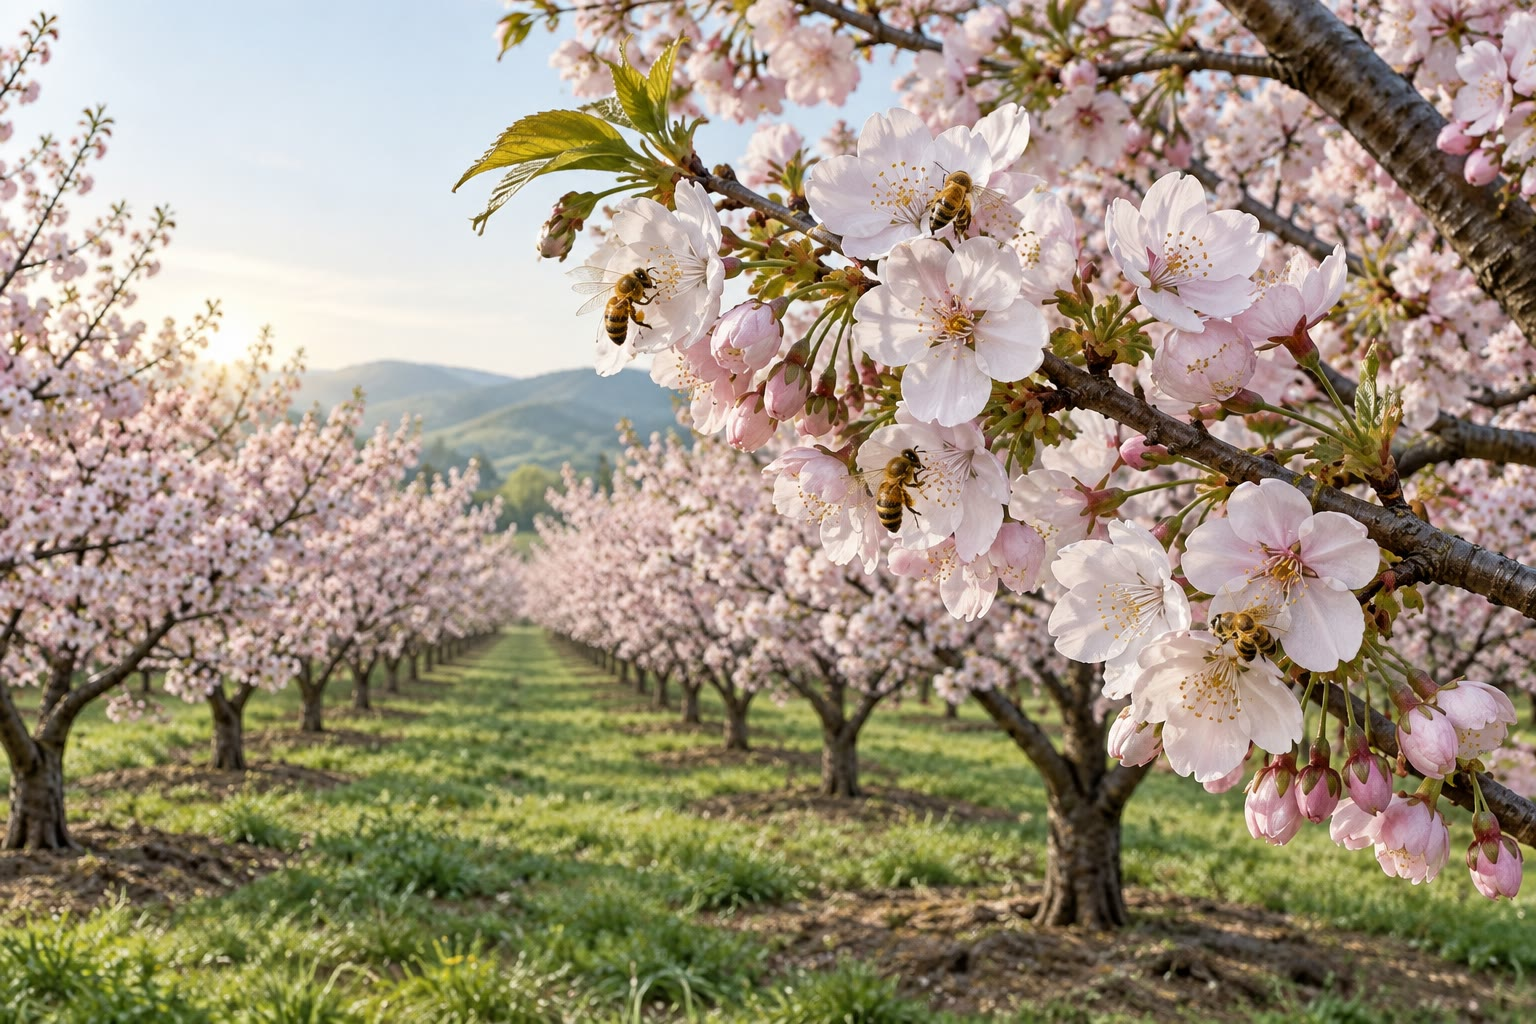
\includegraphics[width=0.62\linewidth]{images/book4/ai/b4-27-phenology-cherry.jpg}

{\small بستان كرز مزهر. فكرز كيوتو، المؤرخ في
اليوميات اثني عشر قرنًا، صار ينفتح أبكر من أي سنة
قبل 1900 --- وعلى النحل الذي يلقّحه أن يطير في
اليوم نفسه.}
\end{omfigure}

\begin{omfigure}
\begin{tikzpicture}
\begin{axis}[
  width=0.74\linewidth, height=5.4cm,
  axis x line=bottom, axis y line=left,
  xmin=0, xmax=100, ymin=0, ymax=14,
  xlabel={الأيام من 1 آذار}, ylabel={الحرارة اليومية المتوسطة (\unit{\celsius})},
  xlabel style={font=\small, at={(axis description cs:0.5,-0.13)}, anchor=north},
  ylabel style={font=\small},
  tick label style={font=\small}, xtick={0,20,40,60,80,100},
  legend style={font=\scriptsize, at={(0.03,0.97)}, anchor=north west, draw=none},
  clip=false,
]
\addplot[very thick, omDef, domain=0:100, samples=2] {2 + 0.1*x};
\addlegendentry{الربيع قبل الاحترار}
\addplot[very thick, omThm, domain=0:100, samples=2] {3 + 0.1*x};
\addlegendentry{ربيع أدفأ بمقدار \qty{1}{\celsius}}
\draw[dashed, gray] (axis cs:0,5) -- (axis cs:100,5); \node[font=\scriptsize, anchor=south east] at (axis cs:100,5) {حرارة الأساس $T_b = \qty{5}{\celsius}$};
\fill[omDef, opacity=0.15] (axis cs:30,5) -- (axis cs:93,5) -- (axis cs:93,11.3) -- cycle;
\fill[omThm, opacity=0.15] (axis cs:20,5) -- (axis cs:83,5) -- (axis cs:83,11.3) -- cycle;
\draw[<->, thick] (axis cs:83,1.6) -- (axis cs:93,1.6); \node[font=\scriptsize, anchor=south] at (axis cs:88,1.8) {10 أيام};
\draw[dotted] (axis cs:93,0) -- (axis cs:93,5); \draw[dotted] (axis cs:83,0) -- (axis cs:83,5);
\node[font=\scriptsize, anchor=south, align=center] at (axis cs:62,11.4) {$K = 200$ درجة-يوم\\ (المساحتان المظللتان)};
\end{axis}
\end{tikzpicture}

{\small درجات-الأيام. يقع الحدث حين تبلغ المساحة المظللة
بين خط الحرارة والأساس $K$؛ وربيع أدفأ بدرجة
واحدة يعبر الأساس قبل عشرة أيام ويتم
المجموع قبل عشرة أيام.}
\end{omfigure}

\section{الخريطة: إزاحات المدى}

\begin{proposition}[خطوط الحرارة تتحرك والأنواع تتبع]\label{prop:b2:global-change:range}
\index{إزاحة المدى}\index{سرعة المناخ}\index{معدل التناقص الحراري}
تهبط الحرارة نحو \qty{6.5}{\celsius} لكل كيلومتر من
الارتفاع ونحو \qty{0.65}{\celsius} لكل مئة كيلومتر من
العرض في المنطقة المعتدلة؛ فاحترار قدره \qty{1}{\celsius}
يحرّك كل خط حرارة نحو \qty{150}{m} صعودًا و
\qty{150}{km} نحو القطب. والأنواع التي تقرر الحرارة حدودها
تتحرك مع خط حرارتها إن استطاعت: فمتوسط مئات
الأنواع المدروسة قد انزاح \qty{11}{m} صعودًا و\qty{17}{km}
نحو القطب في العقد منذ 1970، أي بسرعة خطوط الحرارة، و
أسرعها --- المتنقلة العامة القصيرة العمر --- يسبقها،
في حين لا تستطيع الأشجار، التي تسافر بذورها أمتارًا في السنة، ولا الأنواع التي
هي أصلًا عند القمة أو القطب، اللحاق: فقمة الجبل ليس
لها إلى أين تذهب، وكل درجة من الاحترار تزيل أعلى
\qty{150}{m} من كل مدى. أما الأنواع البحرية، ولا حواجز لها
وحدودها الحرارية أحد، فتتحرك أسرع، أي عشرات الكيلومترات في العقد؛
وقد تحركت القدّية والإسقمري ومصايدهما معهما شمالًا
عبر بحار كاملة. والحافة العليا للمدى تتقدم، والحافة
السفلى تتراجع إذ تدفأ وإذ تصل منافسات جديدة من
الأسفل، ويُعاد تركيب المجتمع في أي نقطة من أنواع
لم تلتق قط.
\end{proposition}
\begin{proof}[شواهد]
أعاد بارميزان (1996) مسح فراشة إديث المرقطة
عبر مداها في غرب أمريكا الشمالية: فوجد جمهرات الحافة
الجنوبية والارتفاعات المنخفضة منقرضة، وجمهرات الحافة الشمالية
والارتفاعات العالية مزدهرة، والمدى كله قد تحرك
\qty{92}{km} شمالًا و\qty{124}{m} صعودًا --- وهو أول نوع بُيّن
أنه تتبع خطوط الحرارة. وقارن لونوار وزملاؤه (2008)
مسوح نبات الغابات لسنوات 1905--1985 بمسوح 1986--2005 عبر
الجبال الفرنسية: فوجدوا الارتفاع الأمثل عند 171 نوعًا قد
ارتفع \qty{29}{m} في العقد. ووجد تشِن وزملاؤه (2011)، عبر
ألفي نوع، الإزاحات أسرع مرتين إلى ثلاث مرات
من التقديرات السابقة، ومتناسبة مع الاحترار الموضعي.
\end{proof}

\begin{omfigure}
\begin{tikzpicture}[every node/.style={font=\scriptsize}, >=stealth]
  \fill[gray!25] (0,0) -- (3.5,4.2) -- (7,0) -- cycle;
  \draw[thick] (0,0) -- (3.5,4.2) -- (7,0);
  \foreach \y/\lab in {1.0/{\qty{12}{\celsius}}, 2.2/{\qty{8}{\celsius}}, 3.4/{\qty{4}{\celsius}}} { \draw[omDef, thick] ({\y/1.2},\y) -- ({7-\y/1.2},\y) node[right] {\lab}; }
  \foreach \y in {1.15,2.35,3.55} { \draw[omThm, thick, dashed] ({\y/1.2},\y) -- ({7-\y/1.2},\y); }
  \node[omThm, anchor=west, align=left] at (7.6,3.7) {المتقطعة: خطوط الحرارة نفسها\\ بعد \qty{1}{\celsius} من الاحترار،\\ أعلى بمقدار \qty{150}{m}};
  \fill[omProp!50] (0.83,1.0) -- (6.17,1.0) -- (5.17,2.2) -- (1.83,2.2) -- cycle;
  \node[align=center] at (3.5,1.6) {نطاق نوع،\\ \qtyrange{1000}{1200}{m}};
  \draw[->, thick, omExo!80!black] (1.1,2.2) -- (1.1,2.9); \node[omExo!80!black, anchor=east, align=right] at (0.95,2.55) {النطاق يصعد\\ ويتقلص};
  \node[anchor=north] at (3.5,-0.1) {جبل: المساحة تتقلص مع الارتفاع، وليس فوق القمة أعلى};
\end{tikzpicture}

{\small إزاحة مدى على جبل. كل درجة ترفع
خطوط الحرارة \qty{150}{m}؛ فيتتبع النوع نطاقه صعودًا إلى
مساحة أصغر، والنطاق الذي هو أصلًا عند القمة يضيع.}
\end{omfigure}

\section{البحر: التحمض والحرارة}

\begin{theorem}[التحمض]\label{thm:b2:global-change:acid}
\index{تحمض المحيط}\index{جملة الكربونات}\index{حالة الإشباع}\index{ابيضاض المرجان}
ثاني أكسيد الكربون المنحل في ماء البحر يصنع حمض الكربون، وهو
يتفكك: $\ensuremath{\mathrm{CO_2}} + \ensuremath{\mathrm{H_2O}} \rightleftharpoons \ensuremath{\mathrm{H^{+}}} +
\ensuremath{\mathrm{HCO_3^{-}}}$، مع $[\ensuremath{\mathrm{H^{+}}}][\ensuremath{\mathrm{HCO_3^{-}}}]/[\ensuremath{\mathrm{CO_2}}] = K_1$.
والبيكربونات أكبر حوض كربون في المحيط وتُبقيها القلوية
شبه ثابتة، فيكون
\[
[\ensuremath{\mathrm{H^{+}}}] \propto p_{\ensuremath{\mathrm{CO_2}}}, \qquad
\Delta\mathrm{pH} \approx -\log_{10}\frac{p_{\ensuremath{\mathrm{CO_2}}}}{p_0}
\]
--- وبدقة أكبر $-0.9\log_{10}$ للنسبة، لأن البيكربونات
ترتفع قليلًا. فمن 280 إلى \qty{420}{ppm} هبطت حموضة السطح
بمقدار $0.15$، من $8.2$ إلى $8.05$: أي زيادة \qty{40}{\%} في شوارد
الهدروجين؛ وعند \qty{800}{ppm} كانت ستهبط $0.4$. وشوارد الهدروجين
الزائدة تستهلك الكربونات، $\ensuremath{\mathrm{H^{+}}} + \ensuremath{\mathrm{CO_3^{2-}}} \to \ensuremath{\mathrm{HCO_3^{-}}}$، و
\emph{\omterm{thm:b2:global-change:acid}{حالة الإشباع}} $\Omega$ لكربونات الكالسيوم ---
أي جداء تركيزي الكالسيوم والكربونات على
جداء الانحلالية --- تهبط بالتناسب: فالأصداف والهياكل
من الأراغونيت (المرجان والجناحيات الأقدام) تتكون بيسر عند $\Omega > 3$، وبعسر
قرب 1، وتنحل دونه؛ والسطح المداري،
وكان $\Omega \approx 4$ قبل الصناعة و3 الآن، يبلغ 2 عند
\qty{560}{ppm}، والمياه القطبية السطحية الباردة الغنية بغاز \ensuremath{\mathrm{CO_2}}
تبلغ 1 أولًا.
\end{theorem}
\begin{proof}
من التوازن يكون $[\ensuremath{\mathrm{H^{+}}}] = K_1[\ensuremath{\mathrm{CO_2}}]/[\ensuremath{\mathrm{HCO_3^{-}}}]$ و
$[\ensuremath{\mathrm{CO_2}}]$ متناسبًا مع $p_{\ensuremath{\mathrm{CO_2}}}$ بقانون هنري؛
ومع بقاء $[\ensuremath{\mathrm{HCO_3^{-}}}]$ ثابتًا، يكون $[\ensuremath{\mathrm{H^{+}}}]$ متناسبًا مع
$p_{\ensuremath{\mathrm{CO_2}}}$ وتتغير $\mathrm{pH} = -\log_{10}[\ensuremath{\mathrm{H^{+}}}]$ بمقدار
$-\log_{10}$ للنسبة. والتوازن الثاني، $[\ensuremath{\mathrm{H^{+}}}][\ensuremath{\mathrm{CO_3^{2-}}}]/[\ensuremath{\mathrm{HCO_3^{-}}}]
= K_2$، يعطي $[\ensuremath{\mathrm{CO_3^{2-}}}] \propto 1/[\ensuremath{\mathrm{H^{+}}}] \propto
1/p_{\ensuremath{\mathrm{CO_2}}}$، فتهبط $\Omega$ كلما ارتفع $p_{\ensuremath{\mathrm{CO_2}}}$، و
ارتفاع $[\ensuremath{\mathrm{H^{+}}}]$ بمقدار \qty{40}{\%} هو هبوط \qty{30}{\%} في
الكربونات. (والكيمياء التامة، مع تغير البيكربونات
وفعاليات الشوارد، تعطي العامل $0.9$ والأعداد
الملحوظة؛ ويعالجها مجلد السنة الثالثة.)
\end{proof}
\begin{proof}[شواهد]
قاست المحطة المحيطية شمال هاواي حموضة السطح شهريًا
منذ 1988: فهي تهبط $0.0018$ في السنة، على وتيرة
\ensuremath{\mathrm{CO_2}} في مونا لوا فوقها، كما تقتضي الكيمياء.
والجناحيات الأقدام --- وهي حلزونات البحر، وغذاء السلمون والحيتان ---
المجموعة قبالة ساحل المحيط الهادئ تُظهر أصدافها الأراغونيتية
منقورة ومنحلة حيث يجلب الصعود المائي ماءً فيه $\Omega <
1$ إلى السطح. أما \omterm{thm:b2:global-change:acid}{ابيضاض المرجان} فحرارة لا حمض: فحين
يبقى الماء \qty{1}{\celsius} فوق الأقصى الصيفي بضعة
أسابيع، يطرد المرجان طحالبه المتعايشة ويجوع؛ وقد ابيض الحاجز
المرجاني العظيم في 1998 و2002 و2016 و2017 و2020 و2022 و2024،
وزال نصف غطائه المرجاني منذ 1995.
\end{proof}

\begin{omfigure}
\begin{tikzpicture}
\begin{axis}[
  width=0.68\linewidth, height=5.4cm,
  axis x line=bottom, axis y line=left,
  xmin=250, xmax=1000, ymin=7.6, ymax=8.3,
  xlabel={\ensuremath{\mathrm{CO_2}} الجوي (\unit{ppm})}, ylabel={حموضة السطح},
  xlabel style={font=\small, at={(axis description cs:0.5,-0.13)}, anchor=north},
  ylabel style={font=\small},
  tick label style={font=\small}, xtick={280,420,560,800,1000}, ytick={7.6,7.8,8.0,8.2},
  clip=false,
]
\addplot[very thick, omDef, domain=250:1000, samples=60] {8.2 - 0.9*log10(x/280)};
\fill[omDef] (axis cs:280,8.2) circle (2pt); \node[font=\scriptsize, anchor=south west] at (axis cs:285,8.2) {1750};
\fill[omThm] (axis cs:420,8.04) circle (2pt); \node[font=\scriptsize, anchor=south west] at (axis cs:425,8.04) {عشرينيات هذا القرن: $-0.15$، $+\qty{40}{\%}$ من \ensuremath{\mathrm{H^{+}}}};
\fill[omThm] (axis cs:800,7.79) circle (2pt); \node[font=\scriptsize, anchor=south west] at (axis cs:805,7.79) {سنة 2100 عند انطلاقات عالية};
\node[font=\scriptsize, anchor=north east, align=right] at (axis cs:1000,8.28) {$\Omega_{\text{الأراغونيت}}$ في المناطق المدارية:\\ 4 سنة 1750، و3 الآن، و2 عند \qty{560}{ppm}};
\end{axis}
\end{tikzpicture}

{\small حموضة سطح المحيط في مقابل ثاني أكسيد الكربون الجوي،
$\mathrm{pH} = 8.2 - 0.9\log_{10}(p/280)$. والمقياس
لوغاريتمي: فكل عُشر وحدة ربع أكثر من شوارد
الهدروجين.}
\end{omfigure}

\begin{omfigure}
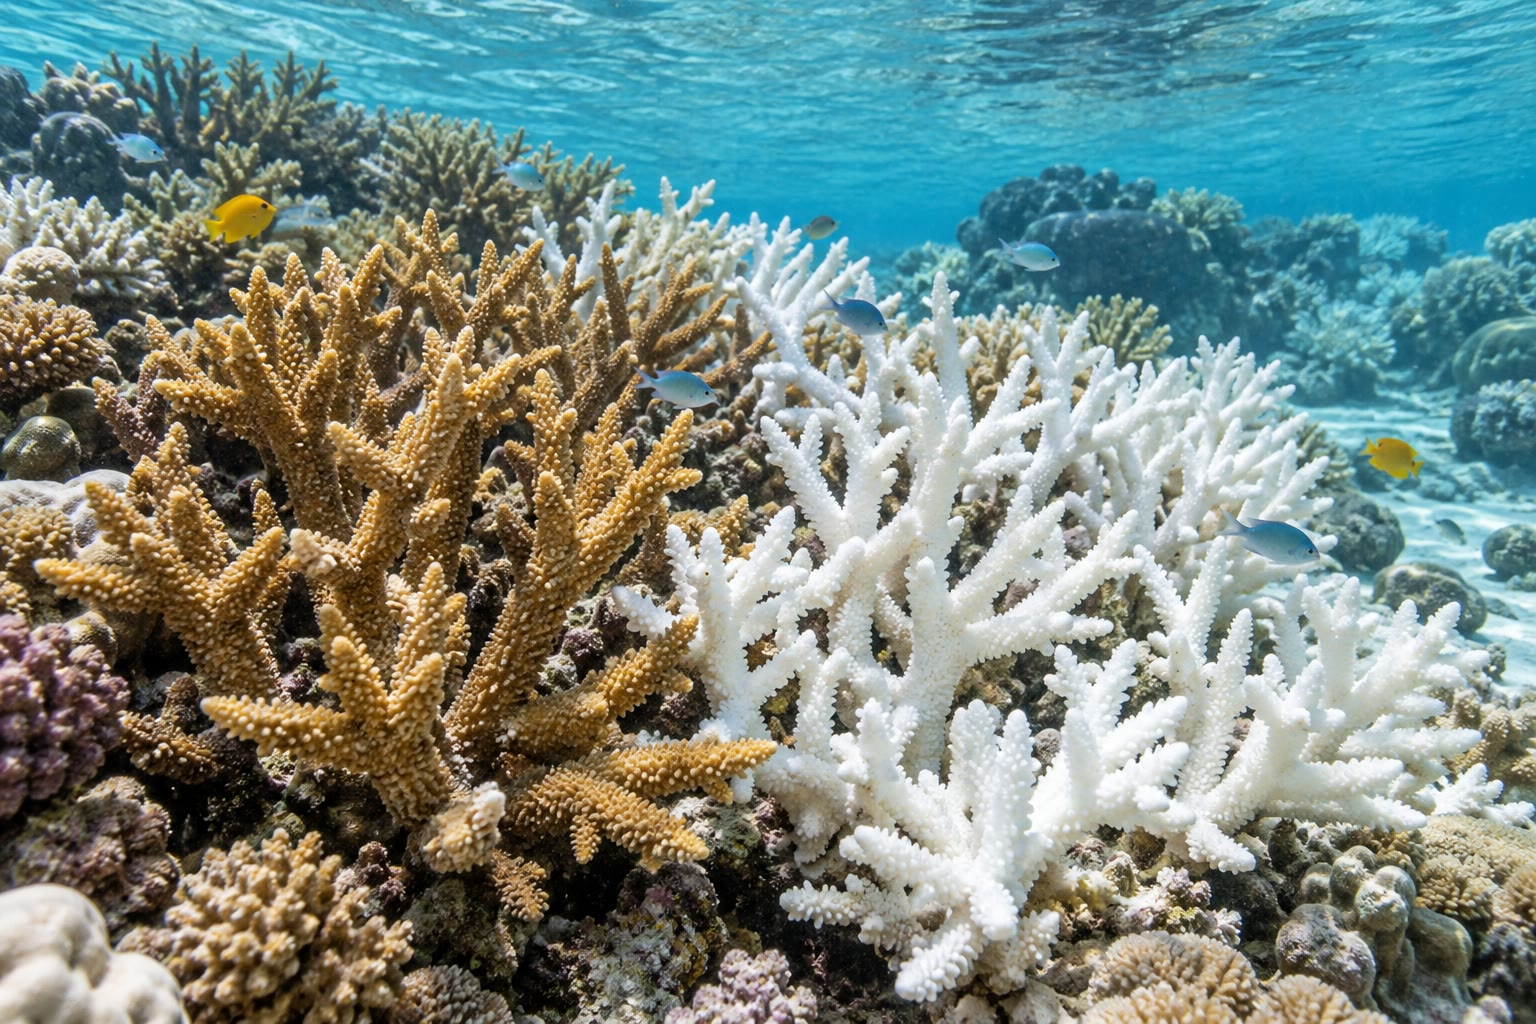
\includegraphics[width=0.44\linewidth]{images/book4/ai/b4-27-coral-bleaching.jpg}\hspace{0.04\linewidth}
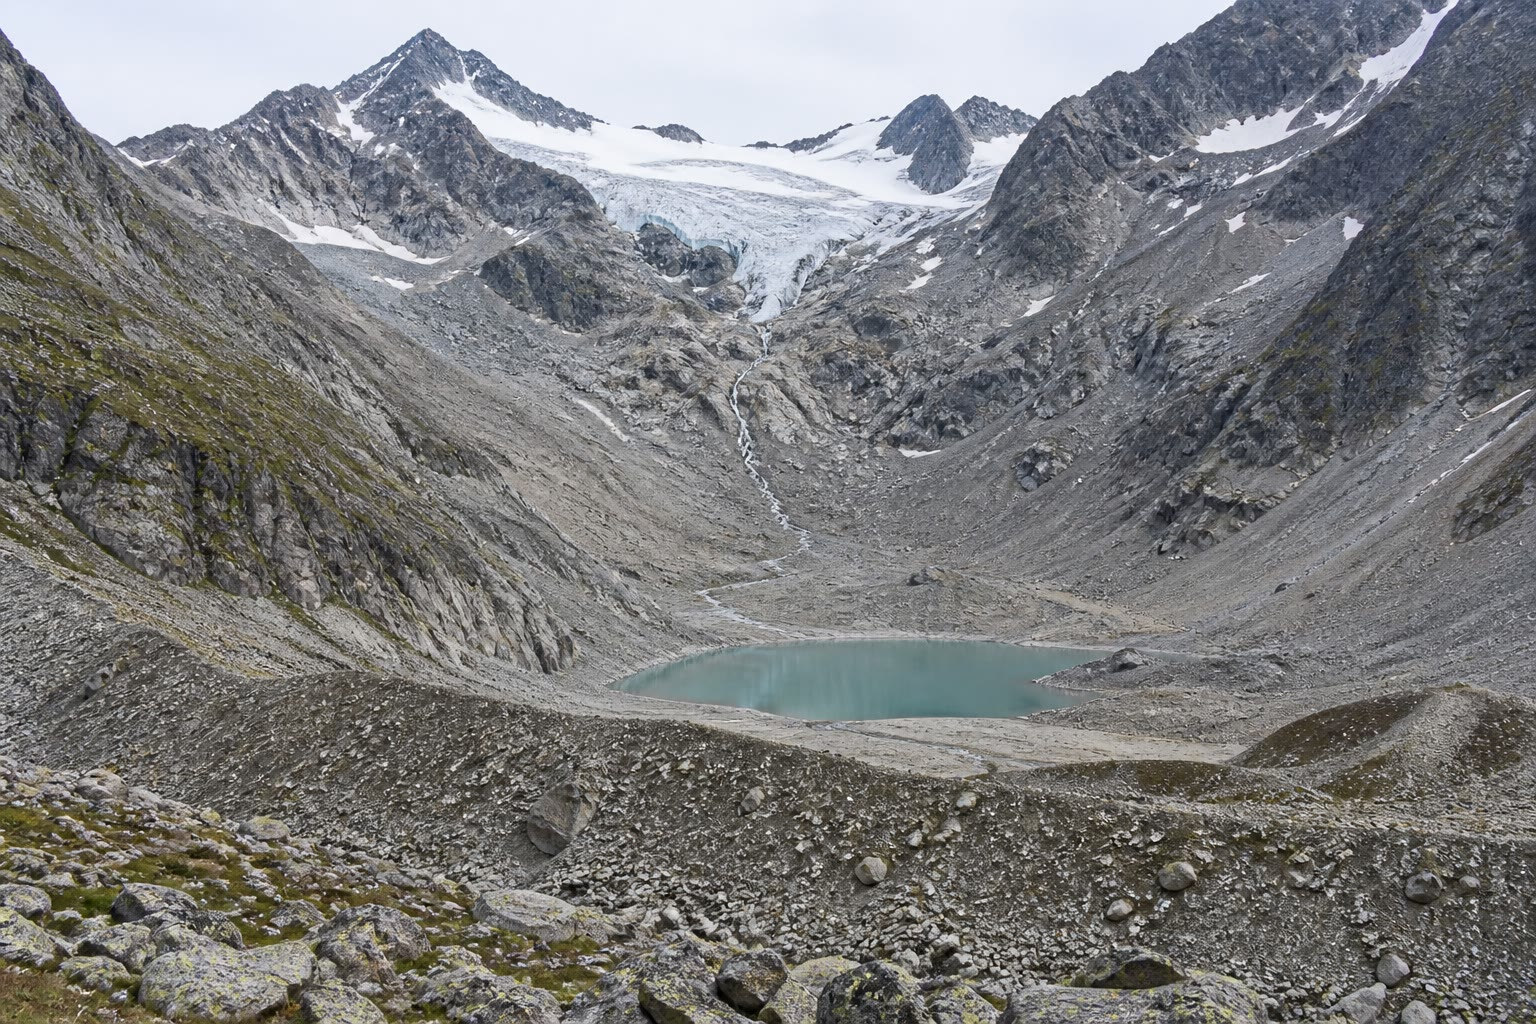
\includegraphics[width=0.44\linewidth]{images/book4/ai/b4-27-glacier-retreat.jpg}

{\small ميزانا حرارة. إلى اليسار: شعاب مبيضّة، وهيكل المرجان
الأبيض يظهر عبر نسيج فقد طحالبه. وإلى اليمين:
نهر جليدي وادٍ انسحب صاعدًا في واديه، تاركًا صخرًا عاريًا
حيث وقف الجليد قبل قرن.}
\end{omfigure}

\section{الدفتر: الانقراض وتقديره}

\begin{theorem}[علاقة الأنواع بالمساحة وكلفة فقد الموئل]\label{thm:b2:global-change:sar}
\index{علاقة الأنواع بالمساحة}\index{معدل الانقراض}\index{فقد الموئل}\index{دين الانقراض}
عدد الأنواع الموجودة في مساحة $A$ ينمو كقوة من
المساحة، $S = cA^{z}$، عند $z \approx 0.25$ للجزر وشُدف
الموائل (فمضاعفة المساحة تضيف خُمسًا من الأنواع؛ ومساحة
أكبر بمئة ضعف تعطي ثلاثة أمثال). وإذا رُدّ موئل
إلى كسر $1 - h$ من امتداده، هبط عدد الأنواع
الذي يستطيع حمله في النهاية إلى $(1 - h)^{z}$ من الأصل: ففقد
نصف الموئل يكلف \qty{16}{\%} من أنواعه، و
\qty{90}{\%} تكلف \qty{44}{\%}، و\qty{99}{\%} تكلف
\qty{68}{\%}. والفقد ليس فوريًا --- فالناجون في
الشُدفة يدومون حينًا، وهو \emph{دين انقراض} يُسدَّد على مدى
عقود إذ تستسلم الجمهرات الصغيرة للانجراف \omterm{prop:b2:population-genetics:inbreeding}{والتزاوج الداخلي} في
\cref{ch:b2:population-genetics} --- وهو أساس
التقدير القائل إن \omterm{thm:b2:global-change:sar}{معدل الانقراض} الحالي مئة إلى
ألف ضعف المعدل الخلفي في السجل الأحفوري: أي نحو
نوع من مليون في السنة، في مقابل عدة آلاف في
السنة، من نحو عشرة ملايين، تُفقد الآن.
\end{theorem}
\begin{proof}
$S'/S = (A'/A)^{z} = (1 - h)^{z}$؛ فعند $z = 0.25$ يكون $0.5^{0.25} =
0.84$، و$0.1^{0.25} = 0.56$، و$0.01^{0.25} = 0.32$. والعلاقة
نفسها تجريبية؛ ويعكس أسّها الميزان، في الجزر،
بين هجرة الأنواع الجديدة الوافدة (وهي تهبط كلما امتلأت الجزيرة)
وانقراض الأنواع المقيمة (وهو يرتفع كلما تقلصت
جمهراتها مع المساحة)، أي توازن نظرية ماك آرثر
وويلسون.
\end{proof}
\begin{proof}[شواهد]
جزر مجموعة كراكاتوا، وقد عُقّمت بثوران
1883، أعاد استعمارها النباتُ والطير والحشرات في
تعاقب بلغ، في غضون خمسين سنة، أعداد الأنواع
المتنبأ بها من مساحاتها؛ والجزيرات الشورانية التي بخّرها سيمبرلوف
وويلسون في فلوريدا سنة 1966 عادت إلى أعداد أنواعها
الأصلية، بأنواع مختلفة، في غضون سنة. والغابة الأطلسية
في البرازيل، وقد رُدّت إلى \qty{10}{\%} من امتدادها، فقدت
أو كادت تفقد كسر أنواع طيورها الذي تتنبأ به العلاقة؛
وفي كل مجموعة قيّمها الاتحاد الدولي لحفظ
الطبيعة يكون ربع الأنواع إلى ثلثها مهددًا --- فالطيور
\qty{13}{\%}، والثدييات \qty{27}{\%}، والبرمائيات \qty{41}{\%}، والمرجان
\qty{44}{\%} --- \omterm{thm:b2:global-change:sar}{وفقد الموئل} السبب الأول، والصيد
والأنواع الغازية والتلوث والمناخ، بصورة متزايدة، أسبابها الأخرى.
\end{proof}

\begin{omfigure}
\begin{tikzpicture}
\begin{loglogaxis}[
  width=0.68\linewidth, height=5.4cm,
  axis x line=bottom, axis y line=left,
  xmin=1, xmax=100000, ymin=5, ymax=200,
  xlabel={مساحة الجزيرة (\unit{km^2})}, ylabel={أنواع طيور اليابسة},
  xlabel style={font=\small, at={(axis description cs:0.5,-0.13)}, anchor=north},
  ylabel style={font=\small},
  tick label style={font=\small},
  clip=false,
]
\addplot[only marks, mark=*, mark size=2pt, omDef] coordinates {(1.5,9) (8,14) (35,22) (150,32) (400,37) (1200,52) (4000,70) (13000,92) (35000,125) (85000,160)};
\addplot[very thick, omThm, domain=1:100000, samples=2] {9*x^0.25};
\node[font=\scriptsize, omThm, anchor=north west, align=left] at (axis cs:2,120) {$S = 9A^{0.25}$: فمساحة أكبر\\ بمئة ضعف تعطي ثلاثة\\ أمثال الأنواع};
\end{loglogaxis}
\end{tikzpicture}

{\small \omterm{thm:b2:global-change:sar}{علاقة الأنواع بالمساحة}، وهي هنا لطيور اليابسة على جزر
أرخبيل: أي خط مستقيم ميله $z = 0.25$ على
محورين لوغاريتميين. فاقطع موئلًا إلى العُشر يبقِ، مع الزمن،
أكثر قليلًا من نصف أنواعه.}
\end{omfigure}

\begin{proposition}[الغزوات والخدمات وما يمكن فعله]\label{prop:b2:global-change:invasion}
\index{نوع غازٍ}\index{خدمات النظام البيئي}\index{تخفيف}\index{صفر صافٍ}
نقلت السفن والطائرات والتجارة آلاف الأنواع عبر
الحواجز التي أبقتها متفرقة؛ ومعظمها يخفق في التوطن، لكن
القليل الذي ينجح --- الأرنب في أستراليا، وبلح البحر المخطط في
البحيرات الكبرى، وأفعى الشجر البنية التي أفرغت غوام من طيورها،
والفطر الكيتريدي الذي دفع تسعين نوعًا برمائيًا إلى
الانقراض --- ينتشر جبهةً تتقدم بسرعة ثابتة، $c =
2\sqrt{rD}$ لجمهرة تنمو بمعدل $r$ وتنتشر
بمعامل انتشار $D$ (فجرذ المسك عند سكيلام، وقد أُطلق قرب
براغ سنة 1905، توسع عبر أوروبا بمقدار \qty{11}{km} في السنة،
ونصف قطر مداه خط مستقيم في الزمن). وفي مقابل هذا كله يقف
ما يفعله المحيط الحيوي لنوعه المزعج الواحد:
تلقيح ثلاثة أرباع المحاصيل، وتنقية الماء، والتحكم
في الفيضان، \omterm{prop:b2:biogeochemical-cycles:nitrogen}{وتثبيت النتروجين} وصنع \omterm{def:b2:living-soil:soil}{التربة}، والمصايد،
والكربون المحبوس في الغابات والترب --- وهي \emph{\omterm{prop:b2:global-change:invasion}{خدمات النظام البيئي}}
المقدَّرة، حيث يمكن وضع ثمن لها، بأكثر من الناتج
الاقتصادي العالمي. وما يمكن فعله يتبع من الأعداد.
فالاحترار يتوقف حين تتوقف الانطلاقات الصافية، لا قبل ذلك: فنماذج
الصندوق في \cref{ch:b2:biogeochemical-cycles} لا تتيح أي قراءة
أخرى \emph{للصفر الصافي}. والأرض تستطيع المساعدة في حدود --- أي
غيغاطن كربون في السنة من إعادة التشجير والترب لبضعة
عقود، في مقابل عشرة من الوقود الأحفوري --- والأنواع يمكن أن
تُعان على الانتقال، أو تُحفظ في محميات كبيرة ومتصلة بما يكفي
حتى لا تُنهيها \omterm{thm:b2:global-change:sar}{علاقة الأنواع بالمساحة} ولا انجراف الجمهرات
الصغيرة. والأدوات هي أدوات هذا الكتاب:
وراثة جمهرات المحمية، ومنافسة الغازي،
وتوقيت المحصول الحيوي، وميزانية \omterm{def:b2:living-soil:soil}{التربة}.
\end{proposition}

\begin{example}[ثلاثة مستقبلات]\label{ex:b2:global-change:scenarios}
انطلاقات تبقى عند \qty{10}{GtC} في السنة حتى 2100 تضيف \qty{800}{GtC}
إلى \qty{700}{} المنطلقة أصلًا: أي $1.65\times 1.5 =
\qty{2.5}{\celsius}$ بحلول نهاية القرن وما زالت ترتفع. وانطلاقات
تهبط إلى الصفر بحلول 2070 تضيف نحو \qty{250}{GtC}: أي \qty{1.6}{\celsius}،
ثم تستوي. ومضاعفة الانطلاقات أولًا، كما فعلت عقود القرن
الأولى، تعطي \qty{4}{\celsius} أو أكثر. وأمداء
المنطقة المعتدلة تتحرك \qty{200}{km} أبعد من اليوم في الحالة الأولى
و\qty{60}{km} في الثانية؛ والربيع يأتي قبل خمسة وعشرين
يومًا، أو ستة؛ وحموضة السطح تبلغ $7.8$، أو تبقى قرب
$8.0$؛ وتقديرات الانقراض، وهي تتوقف على الموئل و
الاحترار معًا، تتراوح بين عُشر الأنواع وثلثها.
والفرق بين المستقبلات هو المساحة المتراكمة تحت منحنٍ
واحد، وهي مجموع قرارات لم تُتخذ بعد.
\end{example}

\section{تمارين}

\begin{exercise}[$\star$]\label{exo:b2:global-change:1}
اذكر العلاقة بين الاحترار \omterm{prop:b2:global-change:tcre}{والانطلاقات المتراكمة}، و
احسب الاحترار عند \omterm{prop:b2:global-change:tcre}{انطلاقات متراكمة} قدرها 700 و1000 و
\qty{2000}{GtC}.
\end{exercise}

\begin{exercise}[$\star$]\label{exo:b2:global-change:2}
عرّف درجات-الأيام \omterm{thm:b2:global-change:phenology}{وعدم التزامن التوقيتي}، مع الخاطف
مثالًا.
\end{exercise}

\begin{exercise}[$\star$]\label{exo:b2:global-change:3}
كم تتحرك خطوط الحرارة صعودًا ونحو القطب لكل درجة من
الاحترار، ولماذا لا يستطيع نوع في قمة جبل اللحاق؟
\end{exercise}

\begin{exercise}[$\star$]\label{exo:b2:global-change:4}
فسّر في ثلاث جمل لماذا تخفض إضافة \ensuremath{\mathrm{CO_2}} إلى البحر
حموضته وكربوناته، وأي الكائنات تتضرر.
\end{exercise}

\begin{exercise}[$\star\star$]\label{exo:b2:global-change:5}
احسب \omterm{prop:b2:global-change:tcre}{ميزانية الكربون} الباقية لأجل \qty{1.5}{\celsius} ولأجل
\qty{2}{\celsius} عند $\lambda = \qty{1.65}{\celsius}$ لكل
\qty{1000}{GtC} و\qty{700}{GtC} منطلقة أصلًا؛ وحوّل الاثنتين إلى
سنوات عند \qty{10}{GtC/yr}.
\end{exercise}

\begin{exercise}[$\star\star$]\label{exo:b2:global-change:6}
يدفأ الربيع بمقدار $b = \qty{0.12}{\celsius}$ في اليوم من أساس قدره
\qty{5}{\celsius}؛ وتحتاج فراشة $K = 150$ درجة-يوم. احسب
الأيام من عبور الأساس إلى الخروج، والتقدم عند
احترار قدره \qty{1.5}{\celsius}.
\end{exercise}

\begin{exercise}[$\star\star$]\label{exo:b2:global-change:7}
مدى نبات يمتد \qtyrange{800}{1400}{m} على جبل
ارتفاعه \qty{1800}{m} تنتصف مساحته كل \qty{300}{m} من الارتفاع.
فبعد \qty{3}{\celsius} من الاحترار، أين النطاق وكم
مساحةً فقد؟ وبعد \qty{5}{\celsius}؟
\end{exercise}

\begin{exercise}[$\star\star$]\label{exo:b2:global-change:8}
احسب حموضة السطح وارتفاع تركيز شوارد الهدروجين
عند 560 و800 و\qty{1000}{ppm}، من $\mathrm{pH} = 8.2 -
0.9\log_{10}(p/280)$.
\end{exercise}

\begin{exercise}[$\star\star$]\label{exo:b2:global-change:9}
عند $z = 0.25$، أي كسر من الأنواع يُفقد في النهاية حين
يُتلف \qty{70}{\%} و\qty{95}{\%} و\qty{99.9}{\%} من موئل؟
ولماذا كان الفقد الفوري أصغر؟
\end{exercise}

\begin{exercise}[$\star\star\star$]\label{exo:b2:global-change:10}
غازٍ ينمو بمعدل $r = 0.7$ في السنة وينتشر عند $D =
\qty{20}{km^2/yr}$. احسب سرعة جبهته والزمن اللازم لعبور
بلد عرضه \qty{1000}{km}. وما الذي ينصّف السرعة: تنصيف $r$ أم
تنصيف $D$؟
\end{exercise}

\begin{exercise}[$\star\star\star$]\label{exo:b2:global-change:11}
\omterm{thm:b2:global-change:sar}{معدل الانقراض} الخلفي 1 لكل مليون نوع-سنة
وهناك 8 ملايين نوع. احسب الانقراضات المنتظرة في
السنة وفي القرن عند المعدل الخلفي، وعند ألف ضعفه.
وقارن بالانقراضات الموثقة البالغة عشرة آلاف في القرن
الأخير وعلّق على التباين.
\end{exercise}

\begin{exercise}[$\star\star\star$]\label{exo:b2:global-change:12}
«الاحترار يتوقف حين تتوقف الانطلاقات الصافية.» برهن من نموذج
صندوق الغلاف الجوي ومن تناسب الاحترار مع
\omterm{prop:b2:global-change:tcre}{الانطلاقات المتراكمة}، وقل ما الناقص في الحجة.
\end{exercise}

\section{مسألة: المحيط الحيوي سنة 2100}

\begin{problem}[{مسألة نهاية الأسبوع --- مساران للانطلاقات محمولان
إلى 2100: احترار كل منهما، والربيع الذي يصنعه، والمسافة
التي تقطعها خطوط حرارته، والحمض الذي يضعه في البحر والأنواع
التي يكلفها غابة، وتنتهي إلى الاحترارين وقيمتي الحموضة
وكسر الأنواع المفقودة}]
\label{pb:b2:global-change:1}
المعطيات. $\lambda = \qty{1.65}{\celsius}$ لكل \qty{1000}{GtC}؛
و\qty{700}{GtC} منطلقة بحلول 2020 (باحترار \qty{1.2}{\celsius}). والمسار
A: \qty{10}{GtC/yr} ثابتة حتى 2100. والمسار B: يهبط خطيًا إلى
الصفر سنة 2070. ويدفأ الربيع بمقدار $b = \qty{0.1}{\celsius}$ في اليوم
فوق أساس قدره \qty{5}{\celsius}؛ وتحتاج شجرة $K = 200$
درجة-يوم لتورق، ويصل طائر مهاجر في تاريخ ثابت،
بعد 20 يومًا من إيراق الشجرة سنة 2020. \omterm{prop:b2:global-change:range}{ومعدل التناقص الحراري}
\qty{6.5}{\celsius/km}؛ والتدرج العرضي \qty{0.65}{\celsius}
لكل \qty{100}{km}. والمحيط: $\mathrm{pH} = 8.2 - 0.9\log_{10}(p/280)$؛
و\ensuremath{\mathrm{CO_2}} سنة 2100: \qty{600}{ppm} على المسار A، و\qty{420}{ppm} على المسار B.
ومنطقة غابية مساحتها \qty{e5}{km^2} فيها 400 نوع شجري، و$z = 0.25$،
تفقد \qty{60}{\%} من مساحتها بالإزالة بحلول 2100 على المسار A و
\qty{20}{\%} على المسار B.

\medskip
\noindent\textbf{الجزء الأول --- الاحترار.}
\begin{enumerate}
  \item احسب \omterm{prop:b2:global-change:tcre}{الانطلاقات المتراكمة} سنة 2100 على كل مسار.
  \item احسب الاحترار سنة 2100 على كل مسار.
  \item احسب الاحترار سنة 2050 على كل منهما.
  \item ما معدل الاحترار في العقد على المسار A؟ وقارنه
        بالقيمة الملحوظة \qty{0.2}{\celsius} في العقد.
  \item على المسار B، هل يتوقف الاحترار سنة 2070؟ ولماذا، بحسب
        التناسب؟
  \item أي انطلاق متراكم يوافق \qty{2}{\celsius}،
        وفي أي سنة يعبره المسار A؟
\end{enumerate}

\medskip
\noindent\textbf{الجزء الثاني --- الربيع.}
\begin{enumerate}[resume]
  \item احسب الأيام من عبور الأساس إلى الإيراق سنة 2020.
  \item احسب تقدم الإيراق، نسبةً إلى 2020، سنة 2100
        على كل مسار (والاحترار نسبةً إلى 2020).
  \item تاريخ وصول الطائر لا يتغير. احسب الفجوة
        بين الإيراق والوصول على كل مسار سنة 2100.
  \item اليرقات التي يحتاجها الطائر تبلغ الذروة بعد 15 يومًا من الإيراق
        وتدوم 10 أيام. فعلى أي مسار يظل الطائر يجدها؟
  \item افترض بدل ذلك أن الطائر يتقدم \qty{3}{d} لكل
        درجة. أعد حساب الفجوة على المسار A.
  \item اذكر في جملة واحدة لماذا كان عدم التزامن، لا الاحترار
        نفسه، هو ما يهدد الطائر.
\end{enumerate}

\medskip
\noindent\textbf{الجزء الثالث --- الأمداء.}
\begin{enumerate}[resume]
  \item احسب الإزاحة الارتفاعية والعرضية
        لخطوط الحرارة على كل مسار، نسبةً إلى 2020.
  \item نوع شجري ينتشر \qty{100}{m} في السنة. فهل يستطيع تتبع
        خطوط الحرارة نحو القطب على المسار A؟ وعلى المسار B؟
  \item نوع يشغل \qtyrange{1500}{1800}{m} على جبل ارتفاعه
        \qty{2000}{m}. فعلى المسار A، أين يقع نطاقه
        سنة 2100، وماذا يحدث؟
  \item تنتصف مساحة الجبل كل \qty{300}{m}. احسب
        عامل المساحة الذي يفقده ذلك النوع على المسار B.
  \item سمكة بحرية تتتبع خطوط الحرارة بمقدار \qty{30}{km} في العقد.
        فهل يكفي ذلك على المسار A؟
  \item فسّر لماذا تتراجع الحافة السفلى لمدى حتى حيث
        يستطيع النوع احتمال الحر.
\end{enumerate}

\medskip
\noindent\textbf{الجزء الرابع --- البحر والغابة.}
\begin{enumerate}[resume]
  \item احسب حموضة السطح سنة 2100 على كل مسار، وارتفاع
        تركيز شوارد الهدروجين منذ 1750.
  \item كانت \omterm{thm:b2:global-change:acid}{حالة الإشباع} $\Omega$ للسطح المداري
        4 سنة 1750 وهي تهبط على صورة $[\ensuremath{\mathrm{H^{+}}}]^{-1}$. احسبها سنة 2100
        على كل مسار وقل ماذا تعني للمرجان.
  \item احسب عدد الأنواع الشجرية التي تستطيع المنطقة الغابية
        حملها في النهاية على كل مسار، والعدد المفقود.
  \item يضيف الاحترار خسائر: افترض أن كل درجة فوق 2020 تزيل
        \qty{5}{\%} أخرى من الأنواع الناجية. أعد حساب
        الأنواع الباقية على كل مسار.
  \item أعطِ كسر الأنواع المفقودة من الأنواع 400 على كل مسار.
  \item أي السببين، الإزالة أم الاحترار، يغلب على
        كل مسار؟
  \item اذكر النتيجة: الاحترار والحموضة وكسر
        الأنواع الشجرية المفقودة سنة 2100 على كل مسار.
\end{enumerate}
\end{problem}
